\documentclass[man,12pt,floatsintext,donotrepeattitle]{apa7}

\usepackage[american]{babel}
\usepackage{csquotes}
\usepackage{amsmath,amssymb}
\usepackage{booktabs}
\usepackage{graphicx}
\usepackage{xcolor}
\usepackage[most]{tcolorbox}
\usepackage{hyperref}
\usepackage[style=apa,backend=biber]{biblatex}
\usepackage{xr}
\usepackage{nameref}
\externaldocument{draft8}
\addbibresource{refs.bib}
\hypersetup{
  hidelinks,
  pdftitle={Supplement 5: Apparatus},
  pdfauthor={Joseph Corneli},
  pdfsubject={The search apparatus accompanying Rule-Rewriting Cellular Automata
    and the Edge of Chaos}
}

\newcommand{\sig}{\sigma}
\newcommand{\secref}[1]{\emph{\nameref{#1}}}

\title{Supplement 5: Apparatus}
\shorttitle{Supplement 5: Apparatus}
\author{Joseph Corneli}
\affiliation{}

\begin{document}
\maketitle

% =====================================================================
% Supplement 5 -- the search apparatus ("the miner").  Draft 2026-08-06.
%
% Scope per Joe, 2026-08-06: the miner is a TOOL, not a theory of MetaCAs and
% not a finding for the main text.  It goes here in full, including the pictures
% of how it searched the phase space and found the ridge.  Its honest negative
% -- no self-driving search was achieved -- is the point of the supplement, not
% an admission buried in it.
%
% Referenced from Part IV, sec:exotype-question.
% =====================================================================

\label{supp:miner}

\subsection*{What it is, and why it is here rather than in the main text}

The examples reported in Part~III were located with the help of an apparatus
built to search for them automatically. That apparatus is a tool. It embodies no
claim about MetaCAs, and its results are about the search rather than about the
substrate, so it is documented here in full and referenced from the main text
only where the provenance of an example matters.

It is documented in full for one reason: it did not do what it was built to do,
and the specific ways in which it failed are reusable. The intended object was a
system that adjusts its own operating point using only quantities it can compute at
runtime, toward the coexistence of frozen and moving structure that the main text
calls the third sense of the edge of chaos. What exists is a system that scores a
parameter surface, moves over it under a learned surrogate, and reports where it
went. The step from the second to the first was not taken, and
\hyperref[supp:miner-negative]{the closing subsection} states precisely which
part of it is missing.

\subsection*{The two coordinates}

The apparatus varies two parameters of the selection rule that chooses among
candidate updates at a site.

\emph{Policy precision} $\beta$ grades how sharply a policy is chosen from its
expected free energy: at $\beta \to 0$ selection is uniform over candidates, and
as $\beta$ grows it concentrates on the score-minimising candidate. We write it
$\beta$ throughout this supplement to avoid collision with the causal-currency
gain $\gamma$ of \secref{sec:gain}, which is a different quantity; the
implementation calls it \texttt{policy-precision}.

\emph{Epistemic weight} $\kappa$ scales the information-seeking term of that
score against the goal-directed term. At $\kappa = 0$ the rule is purely
exploitative.

Both are swept geometrically: $\beta \in \{1,2,4,8,16,32,64\}$ and
$\kappa \in \{0, 0.1, 0.2, 0.5, 1\}$, giving thirty-five cells, each run at four
seeds.

\subsection*{The objective, and its validation}

The apparatus scores a run by an intrinsic measure rather than by damage reach,
because damage reach is computed on a twin run and is therefore unavailable to
the system itself. The phenotype spacetime sheet is tiled into $100\times100$
patches, each packed contiguously to a bitstring and compressed; the observable
is the \emph{fraction of patches whose compression ratio lies in $[0.3,0.9]$},
which distinguishes a graded distribution from a bimodal one.

Patch size and packing are both load-bearing and both produced defects worth
recording. At $S=50$ the compressor's own header dominates a $312$-byte payload
and the incompressible end of the scale saturates, so several distinct regimes
score identically at the ceiling. And packing patch rows to whole bytes appends
four zero bits per row, a period-$13$ regularity present in every patch that the
compressor exploits; the first version of the validation table was wrong for
this reason, and correcting it removed an apparent winner.

Validated against elementary rules of undisputed regime, the corrected measure
separates in the intended direction: rules $54$ and $110$ score $94\%$ and
$75\%$, while $204$ (frozen), $90$ (nested) and $30$ (chaotic) all score $0\%$.
It is worth noting that it places rule $90$ with rule $30$, declining to call it
class~IV despite its fractal appearance, where damage reach places rule $90$
next to the frozen rule.

\subsection*{The surface, and the ridge}

Table~\ref{tab:miner-surface} gives the objective over the thirty-five cells.

\begin{table}[htbp]
\centering
\caption{The objective over the search space, averaged over four seeds. Nonzero
values occupy an L-shaped ridge: low $\beta$ at any $\kappa$, and any $\beta$ at
$\kappa \le 0.1$. Everything else is identically zero.}
\label{tab:miner-surface}
\begin{tabular}{rrrrrr}
\toprule
$\beta \backslash \kappa$ & $0.0$ & $0.1$ & $0.2$ & $0.5$ & $1.0$ \\
\midrule
$1$  & 0.594 & \textbf{0.641} & 0.562 & 0.562 & 0.625 \\
$2$  & 0.422 & 0.422 & 0.406 & 0.438 & 0.469 \\
$4$  & 0.312 & 0.219 & 0.109 & 0.250 & 0.000 \\
$8$  & 0.000 & 0.453 & 0.156 & 0.000 & 0.000 \\
$16$ & 0.203 & 0.484 & 0.047 & 0.000 & 0.000 \\
$32$ & 0.609 & \textbf{0.625} & 0.000 & 0.000 & 0.000 \\
$64$ & 0.484 & 0.547 & 0.000 & 0.000 & 0.000 \\
\bottomrule
\end{tabular}
\end{table}

The surface has two arms and a valley between them. One arm runs along low
$\beta$ and survives every value of $\kappa$; the other occupies high $\beta$ at
$\kappa \le 0.1$ and vanishes abruptly at $\kappa = 0.2$. Between them, at
$\beta = 4$ to $16$, the objective falls to a minimum of $0.109$ and in three
cells to zero. Approached from below the ridge is a broad plateau; approached
from above it is a cliff.

This geometry is the useful product of the search, and it is not what the search
was built to produce. Two facts about it are established in the main text and
should be read together with the table. The high-$\beta$ arm consists of
configurations that reach an absorbing state --- $\beta = 32$ at $\kappa = 0.1$
freezes permanently at $t=1046$ --- while the low-$\beta$ arm does not. And the
examples exhibiting criticality lie in the valley, at $\beta = 8$ to $10$,
scoring \emph{below} both arms. The objective's two maxima are a living regime
and a dying one, and it ranks the dying one highest.

\subsection*{The search paths}

Figure~\ref{fig:miner-paths} shows twelve-episode trajectories from four
starting points under a surrogate-driven policy, drawn twice: over the control
space the apparatus manipulates, and over the two-dimensional observable space
in which it perceives its own position.

\begin{figure}[htbp]
\centering
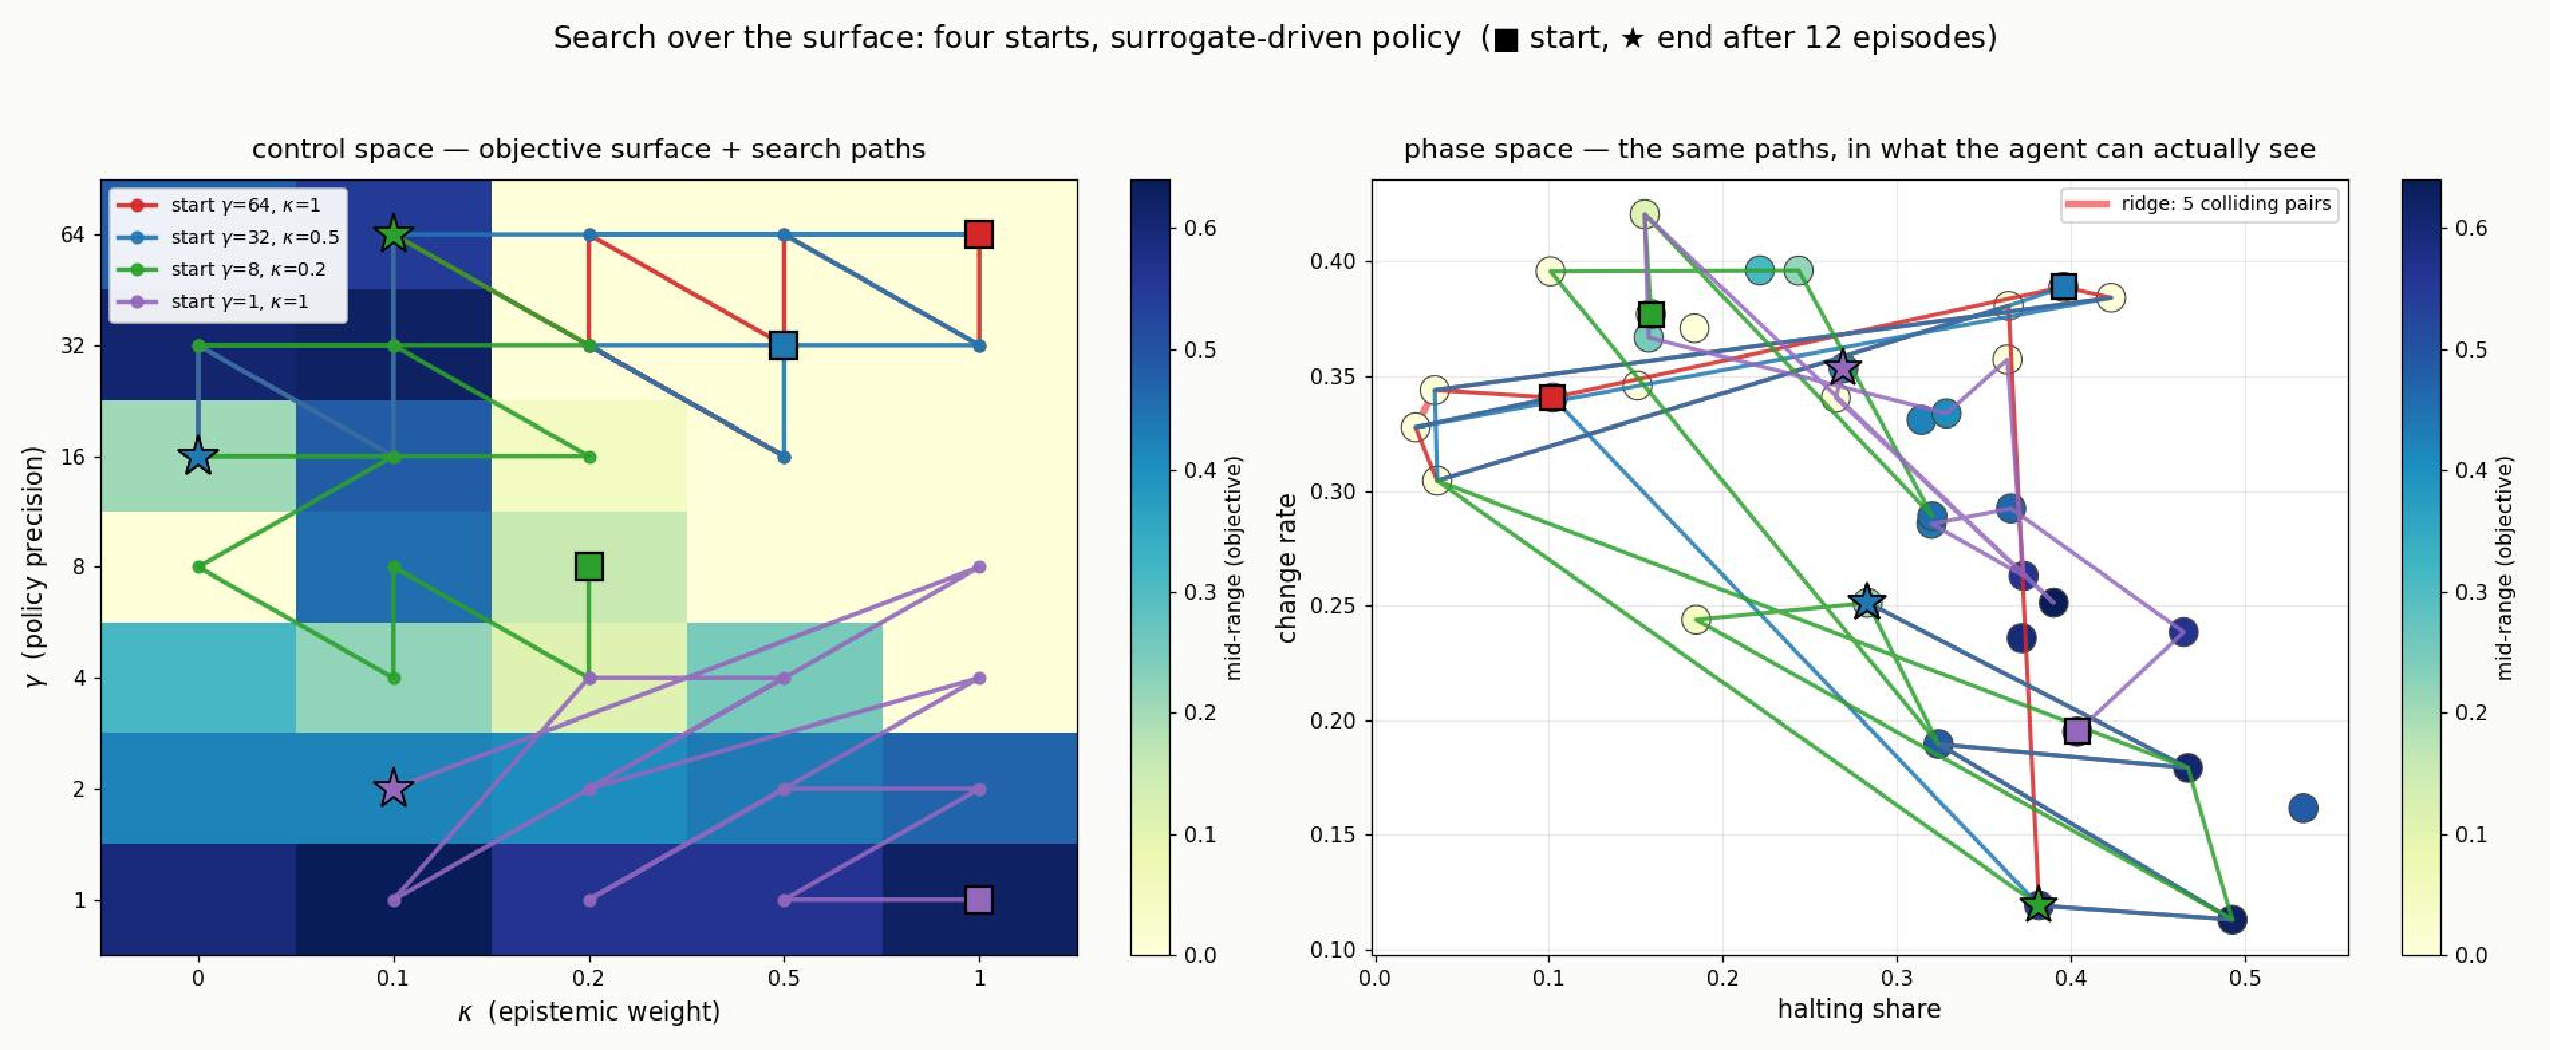
\includegraphics[width=\linewidth]{figures/miner-search-paths.pdf}
\caption{Search over the surface. Left: the objective with four search paths in
control space $(\kappa, \beta)$. Right: the same paths in the observable space
the apparatus can actually see --- halting share against change rate. The marked
ridge joins the five cell pairs that collide within $0.02$ in that space; along
it the apparatus cannot distinguish its own position.}
\label{fig:miner-paths}
\end{figure}

The right-hand panel carries the substantive limitation. Of $595$ cell pairs,
five collide within $0.02$ in observable space --- most consequentially
$(\beta=2, \kappa=0.5)$ with $(\beta=8, \kappa=0.1)$, which the main text shows
to be dynamically very different. A policy reading only these two observables is
blind along that ridge. This is documented rather than repaired.

\subsection*{The screen that should have come first}

An earlier controller in this family targeted a different pair: a knob $\lambda$
weighting a conatus term, with realised winner-hunger as its sensor. Sweeping
$\lambda$ across its entire range moves mean realised hunger by $0.005$, against
a seed-level spread an order of magnitude larger. A closed-loop sweep over ten
target values then found every target settling at a boundary, with a bifurcation
between $0.160$ and $0.170$: below it $\lambda$ runs to one, above it to zero,
and nothing rests between. The critical target was not an attractor but the mean
realised hunger itself, separating positive error forever from negative error
forever. A sign controller on a flat plant has no interior fixed point.

That controller could not have worked, and this was establishable before it was
built. The screen we now apply to any candidate pair $(u, y)$ has four
conditions, each cheap: does $u$ move $y$ on-policy by more than seed noise
(\emph{leverage}); does the target lie inside $y$'s attainable range
(\emph{reachability}); does $y$ track the objective rather than merely being
movable (\emph{validity}); and does the closed loop have a fixed point rather
than a repeller (\emph{stability}). The $\lambda$--hunger pair fails leverage,
fails reachability twice over, and fails stability. Validity was never reached.
Applied to the other knobs, the screen selects $\beta$, which passes the first
three outright --- and $\beta$ had not been treated as a control at all.

\subsection*{The bridge test}

The obstruction that then appears is different in kind from the one $\lambda$
met, and it is the reason the loop remains open. Damage reach is measured by
forking a run, perturbing one bit, advancing a twin and counting divergences. No
system can compute it about itself. So a controller on $\beta$ cannot use the
sensor that makes $\beta$ attractive, and the question becomes whether any
runtime-computable quantity tracks a target worth reaching.

Two leave-one-out tests answer it, and they answer it differently:

\begin{center}
\begin{tabular}{lr}
\toprule
predictors $\to$ target & held-out $R^2$ \\
\midrule
internal score $\to$ damage reach (external, twin-run) & $+0.016$ \\
(halting share, change rate) $\to$ local compressibility (intrinsic) & $+0.726$ \\
\bottomrule
\end{tabular}
\end{center}

Same system, same class of observable, same form of test; the difference is
whether the target is something the system can perceive. The estimator was
smoke-tested on synthetic signal ($+0.976$) and synthetic noise ($-0.165$)
before being run on real data, and the objective column was reproduced
identically across two independently written implementations, so the contrast is
attributable to the system rather than to the analysis. An earlier value of
$+0.541$ for the second row reflected a window mismatch between the observable
and objective runs; measuring both on the matched window recovers $+0.726$.

The conclusion is narrow and worth stating exactly. \textbf{The loop is closable
--- just not on damage reach.} A pair of quantities the system computes anyway
predicts an intrinsic objective well. That result survives the discovery,
reported in the main text, that the objective itself ranks configurations
against their long-run survival, because it is a statement about coupling
between sensor and target rather than about the value of the target.

\subsection*{What was not achieved}
\label{supp:miner-negative}

No self-driving search was built. The apparatus scores a surface and moves over
it; it does not adjust its own operating point toward criticality using only
runtime quantities, and it was never run in a closed loop against a live system.
The examples in Part~III were found by this apparatus together with our own
reading of what it returned --- our choice of which cells to run long, our
noticing that the highest-scoring cells were the ones that died --- and we cannot
separate the two contributions. Where the main text reports an example, it
reports it as an object with measured properties, not as the output of an
autonomous procedure.

Three further gaps are worth recording against any attempt to close the loop.
The objective, as the main text establishes, is not the right target: it rewards
the frozen phase that precedes permanent freezing, and a controller ascending it
would ascend toward death. The observable space is degenerate along the ridge of
Figure~\ref{fig:miner-paths}, so even a correct target would be pursued blind in
that region. And the stability condition of the screen was never tested for
$\beta$, because the target it would have been tested against did not survive.
A controller on this apparatus therefore remains unbuilt for a reason that is
now specific rather than general: not that the system cannot be steered, but
that we do not yet have a target worth steering toward that it can also see.


\subsection*{A second apparatus, for an experiment not run here}

The preceding sections describe a search over an existing construction. This one
describes how a \emph{selection} experiment over the same substrate should be
specified before it is built. The two share a discipline and not a subject: there
the question was whether a knob could move its sensor, here it is whether a
population could exhibit the effect the experiment is built to detect. The
material is retained because the conditions below are checkable in advance, and
because the experiment they govern --- adding a selective filter, so that
plasticity alters what selection sees --- is the extension the main text names and
does not carry out.

\subsection*{Specifying a Selection Experiment Before Running It}
\label{sec:apparatus}

A selection experiment reports trajectories. Nothing in a trajectory says whether
the experiment was capable of exhibiting the effect it was built to detect, and a
run that could not have succeeded produces the same shape of output as one that
tried and failed. The apparatus described here exists to separate those two cases
in advance rather than after the fact.

\subsubsection*{The target as a certificate}

We state the target as an object that must be exhibited, not as a pattern to be
recognised in a plot. A genome carries a rule at each locus together with a flag
marking that locus as held; a held locus keeps its inherited rule for the whole
evaluation. Writing $\mathrm{dep}$ for the dependence of a genome on
within-evaluation rewriting and $\mathrm{perf}$ for its raw function, a completed
assimilation claim is a path $g_0,\dots,g_n$ satisfying, simultaneously:

\begin{enumerate}
\item every step $g_i \to g_{i+1}$ is admitted by the declared genetic operators;
\item $\mathrm{perf}(g_i) \ge \tau$ for every $i$, so the path never leaves the
      functional region;
\item $\mathrm{dep}(g_{i+1}) \le \mathrm{dep}(g_i)$ at every step, and
      $\mathrm{dep}(g_n) < \mathrm{dep}(g_0)$ strictly;
\item $g_n$ is static --- every locus held; and
\item $\mathrm{perf}$ of $g_n$ with every locus held still clears $\tau$.
\end{enumerate}

The last condition is the one most easily omitted. A population can reduce its
measured dependence without its inherited field being able to carry the behaviour
alone, and only an explicit held-rule evaluation distinguishes the two.

Selection, however, does not rank raw function. It ranks fitness
$\mathrm{fit}_c = \mathrm{perf} - c\,\mathrm{dep}$. A path can therefore satisfy
all five conditions and still be untraversable, because a step that preserves
function may lose fitness. Adding the requirement
$\mathrm{fit}_c(g_{i+1}) \ge \mathrm{fit}_c(g_i)$ gives a strictly stronger object,
and makes a conflict explicit that is otherwise rediscovered empirically: a
dependence-reducing step keeps its fitness exactly when
\begin{equation}
\mathrm{perf}(g_i) - \mathrm{perf}(g_{i+1}) \;\le\;
  c\,\bigl(\mathrm{dep}(g_i) - \mathrm{dep}(g_{i+1})\bigr),
\label{eq:selectable}
\end{equation}
that is, when the function a hold costs is no more than the cost it saves. If the
inequality fails at every accessible dependence-reducing step, no traversable path
exists at any length, and \eqref{eq:selectable} identifies $c$ as the parameter that
would dissolve the obstruction.

\subsubsection*{Conditions checkable before the run}

Two consequences are checkable without running anything. First, if dependence takes
a single value across the reachable genomes, the strict-decrease condition cannot be
met and no certificate of any length exists; a constant axis is therefore a
disqualifying property of the design, not a null result. Second, and less obviously,
an axis on which the score is non-constant may still be untraversable: a profile that
is zero at every level but one has two distinct values and a single transition, and a
hill-climber cannot cross a lone cliff. Counting the adjacent transitions that carry
gradient, rather than counting distinct values, is what distinguishes a navigable axis
from a spike.

This distinction is not hypothetical here. Under the gain parameterisation of the main text's
endogenous gate, sampled at eight uniform levels, the band score is zero
at seven of them and positive at the eighth. The design is disqualified by the second
criterion while passing the first, and re-resolving the parameter where the gain curve
is convex is what makes the axis traversable --- a change to the experiment rather
than to the check.

\subsubsection*{Invariants the implementation must satisfy}

The specification above constrains the target. A second family of conditions
constrains the apparatus, and each is stated as an executable predicate tested
against the specific failure that motivated it, since a check written from the
description of an invariant rather than from its counterexample can pass the defect
it was introduced to catch.

\begin{description}
\item[Tape alignment.] Both branches of a perturbation fork must consume identical
  random draws whatever their gates decide. A gate that reads the phenotype fires at
  different loci in the two branches, so a closed gate that skips a draw
  desynchronises the tapes and the divergence that follows is an artefact of the
  generator rather than a causal effect. The discipline is to draw unconditionally and
  then decide how to use the draw; the check must also confirm the branches actually
  differed, since equal draw counts are trivially equal when they do not.
\item[Layering fidelity.] Any extension must reproduce the measurement it extends
  when its additional machinery is in the neutral position. Determinism does not imply
  fidelity: an extension can reproduce byte-for-byte and still report a different value
  than the construction it claims to generalise.
\item[Linked inheritance.] Every heritable component must travel together under
  recombination. Transferring a rule without its held flag places it under an
  unrelated hold pattern, so the operator no longer tests the mechanism it was
  introduced for.
\item[Operator reachability.] Every value of every gene must be attainable under
  mutation. A value the operator cannot reach is present in the representation and
  absent from the experiment.
\item[Empirical null.] Any claim of the form ``rarer than chance'' requires a
  no-selection control running the identical lifecycle. An analytical baseline must
  match the lifecycle actually implemented: with elitist retention, in which survivors
  are not re-mutated, the mutation-only expectation for a symmetric flip rate $\mu$
  after $n$ generations is $\tfrac{1}{2}\bigl(1 - (1-\mu)^n\bigr)$ rather than the
  familiar $\tfrac{1}{2}\bigl(1 - (1-2\mu)^n\bigr)$.
\item[Treatment separation.] Selection ranks scores, so a term that shifts every
  genome equally cannot act. Arms differing in such a term will coincide, and their
  coincidence is a diagnostic of an inert treatment rather than a robust result.
\end{description}

Two of these deserve emphasis because they invert a natural reading. The empirical
null is not a formality: in the runs reported here, dependence falls and the held
fraction rises under no selection at all, purely because holds accumulate by
mutation. Declining dependence is therefore not evidence of assimilation, and a
treatment must be compared against that trajectory rather than against zero.
Treatment separation is the complementary case: identical arms indicate that the
parameter never reached selection.

\subsubsection*{Diagnosing a negative result}

When a run produces no certificate, the specification does not say why, and the three
possible reasons call for different remedies. Holding each locus of a high-performing
plastic genome at each admissible rule separates them. If no rule preserves function
at a locus, the plastic computation there is not representable by any single static
rule. If some rule preserves function but the inherited allele does not, the
representation suffices and the difficulty is that mutation cannot prepare the allele
before it is fixed. If the inherited allele itself preserves function and improves
fitness, an assimilation step was available and the search did not take it. Only the
first is a statement about the substrate.

The distinction is decidable cheaply. Testing each locus at its current allele costs
one evaluation per locus rather than one per locus and rule, and settles the third
case outright when it fires.

\subsubsection*{What the apparatus does not establish}

These conditions are necessary, not sufficient. They constrain what an experiment can
claim; they do not make its measurements correct, and no invariant here would detect a
mis-specified dynamics that satisfies all of them. They are also specific to the
construction studied in Part~III: the certificate assumes a genome with per-locus
holding and a scalar cost, and neither the conditions nor the diagnostic transfers
unchanged to a different architecture. Finally, the calibration used by the score must
share dynamics with the constructions placed on it; boundary conditions that differ
between a calibration and the objects it calibrates can reorder the reference rules
themselves, and where that holds the resulting band assignments are not comparable.

\printbibliography
\end{document}
